\documentclass{tufte-handout}

\title{Szemerédi Regularity Lemma}

\author[Aaksh Ghosh]{Aakash Ghosh(19MS129)}

%\date{28 March 2010} % without \date command, current date is supplied

%\geometry{showframe} % display margins for debugging page layout

\usepackage{graphicx} % allow embedded images
	\setkeys{Gin}{width=\linewidth,totalheight=\textheight,keepaspectratio}
	\graphicspath{{graphics/}} % set of paths to search for images
\usepackage{amsmath}  % extended mathematics
\usepackage{booktabs} % book-quality tables
\usepackage{units}    % non-stacked fractions and better unit spacing
\usepackage{multicol} % multiple column layout facilities
\usepackage{lipsum}   % filler text
\usepackage{fancyvrb} % extended verbatim environments
	\fvset{fontsize=\normalsize}% default font size for fancy-verbatim environments

% Standardize command font styles and environments
\newcommand{\doccmd}[1]{\texttt{\textbackslash#1}}% command name -- adds backslash automatically
\newcommand{\docopt}[1]{\ensuremath{\langle}\textrm{\textit{#1}}\ensuremath{\rangle}}% optional command argument
\newcommand{\docarg}[1]{\textrm{\textit{#1}}}% (required) command argument
\newcommand{\docenv}[1]{\textsf{#1}}% environment name
\newcommand{\docpkg}[1]{\texttt{#1}}% package name
\newcommand{\doccls}[1]{\texttt{#1}}% document class name
\newcommand{\docclsopt}[1]{\texttt{#1}}% document class option name
\newenvironment{docspec}{\begin{quote}\noindent}{\end{quote}}% command specification environment

\usepackage{amsthm}

\newtheorem{theorem}{Theorem}[]
\newtheorem{definition}{Definition}[]
\newtheorem{corollary}{Corollary}[theorem]
\newtheorem{lemma}[theorem]{Lemma}

\setcounter{secnumdepth}{-1}

\usepackage{physics}
\usepackage{amsmath}
\usepackage{tikz}
\usepackage{mathdots}
\usepackage{yhmath}
\usepackage{cancel}
\usepackage{color}
\usepackage{array}
\usepackage{multirow}
\usepackage{amssymb}
\usepackage{gensymb}
\usepackage{tabularx}
\usepackage{extarrows}
\usepackage{booktabs}
\usetikzlibrary{fadings}
\usetikzlibrary{patterns}
\usetikzlibrary{shadows.blur}
\usetikzlibrary{shapes}

\begin{document}
\maketitle% this prints the handout title, author, and date

\begin{abstract}
\noindent
\end{abstract}
Let $G$ be a graph and let $A$ and $B$ be disjoint set of vertices of $G$. Let $e(A,B)$ be the number of edges from $A$ to $B$. Define $d(A,B)=\frac{e(A,B)}{|A||B|}$  \sidenote{Note that $d(A,B)$ is a somewhat normalised measure of how well two vertex set is connected  with each other. The value of $d$ will range from 0(i.e no connection) to 1(i.e all possible edges are present and very well connected)}


\begin{lemma}
	If $y\in[a,b]$ then
	\begin{align}
	|x-y|\leq c\Leftrightarrow |x-a|\leq c,|x-b|\leq c
	\end{align}
\end{lemma}
\begin{proof}
There are three possible cases as shown in Fig 1. The blue line shows the valuesw $y$ takes.

\end{proof}




\begin{theorem}
	If $X\subset A$ and $Y\subset B$ with $\frac{|X|}{|A|}\geq 1-\delta$ and $\frac{|Y|}{|B|}\geq 1-\delta$ where $0\leq \delta\leq\frac{1}{2}$. Then:
	\begin{align}
	|d(X,Y)-d(A,B)|\leq 2\delta\\
	|d^2(X,Y)-d^2(A,B)|\leq 4\delta
	\end{align}
\end{theorem}\noindent
\begin{marginfigure}


	\tikzset{every picture/.style={line width=0.75pt}} %set default line width to 0.75pt

	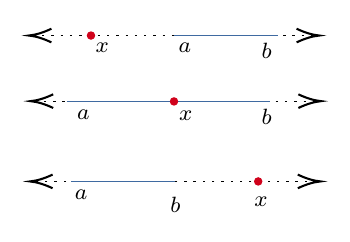
\begin{tikzpicture}[x=0.75pt,y=0.75pt,yscale=-1,xscale=1]
	%uncomment if require: \path (0,300); %set diagram left start at 0, and has height of 300

	%Straight Lines [id:da44850145401460706]
	\draw  [dash pattern={on 0.84pt off 2.51pt}]  (92.86,81.61) -- (228.86,81.61) ;
	\draw [shift={(230.86,81.61)}, rotate = 180] [color={rgb, 255:red, 0; green, 0; blue, 0 }  ][line width=0.75]    (10.93,-3.29) .. controls (6.95,-1.4) and (3.31,-0.3) .. (0,0) .. controls (3.31,0.3) and (6.95,1.4) .. (10.93,3.29)   ;
	\draw [shift={(90.86,81.61)}, rotate = 0] [color={rgb, 255:red, 0; green, 0; blue, 0 }  ][line width=0.75]    (10.93,-3.29) .. controls (6.95,-1.4) and (3.31,-0.3) .. (0,0) .. controls (3.31,0.3) and (6.95,1.4) .. (10.93,3.29)   ;
	%Straight Lines [id:da44467407695726846]
	\draw [color={rgb, 255:red, 63; green, 106; blue, 161 }  ,draw opacity=1 ]   (108.29,81.61) -- (206.29,81.61) ;
	%Straight Lines [id:da03160934519071412]
	\draw  [dash pattern={on 0.84pt off 2.51pt}]  (92,50) -- (228,50) ;
	\draw [shift={(230,50)}, rotate = 180] [color={rgb, 255:red, 0; green, 0; blue, 0 }  ][line width=0.75]    (10.93,-3.29) .. controls (6.95,-1.4) and (3.31,-0.3) .. (0,0) .. controls (3.31,0.3) and (6.95,1.4) .. (10.93,3.29)   ;
	\draw [shift={(90,50)}, rotate = 0] [color={rgb, 255:red, 0; green, 0; blue, 0 }  ][line width=0.75]    (10.93,-3.29) .. controls (6.95,-1.4) and (3.31,-0.3) .. (0,0) .. controls (3.31,0.3) and (6.95,1.4) .. (10.93,3.29)   ;
	%Shape: Circle [id:dp5333382021730819]
	\draw  [color={rgb, 255:red, 208; green, 2; blue, 27 }  ,draw opacity=1 ][fill={rgb, 255:red, 208; green, 2; blue, 27 }  ,fill opacity=1 ] (118.25,50) .. controls (118.25,49.03) and (119.03,48.25) .. (120,48.25) .. controls (120.97,48.25) and (121.75,49.03) .. (121.75,50) .. controls (121.75,50.97) and (120.97,51.75) .. (120,51.75) .. controls (119.03,51.75) and (118.25,50.97) .. (118.25,50) -- cycle ;
	%Straight Lines [id:da028463898146168343]
	\draw [color={rgb, 255:red, 63; green, 106; blue, 161 }  ,draw opacity=1 ]   (160,50) -- (210,50) ;
	%Shape: Circle [id:dp2813904121246703]
	\draw  [color={rgb, 255:red, 208; green, 2; blue, 27 }  ,draw opacity=1 ][fill={rgb, 255:red, 208; green, 2; blue, 27 }  ,fill opacity=1 ] (158.25,81.75) .. controls (158.25,80.78) and (159.03,80) .. (160,80) .. controls (160.97,80) and (161.75,80.78) .. (161.75,81.75) .. controls (161.75,82.72) and (160.97,83.5) .. (160,83.5) .. controls (159.03,83.5) and (158.25,82.72) .. (158.25,81.75) -- cycle ;
	%Straight Lines [id:da2300956631550083]
	\draw  [dash pattern={on 0.84pt off 2.51pt}]  (228.57,120.29) -- (92.57,120.29) ;
	\draw [shift={(90.57,120.29)}, rotate = 360] [color={rgb, 255:red, 0; green, 0; blue, 0 }  ][line width=0.75]    (10.93,-3.29) .. controls (6.95,-1.4) and (3.31,-0.3) .. (0,0) .. controls (3.31,0.3) and (6.95,1.4) .. (10.93,3.29)   ;
	\draw [shift={(230.57,120.29)}, rotate = 180] [color={rgb, 255:red, 0; green, 0; blue, 0 }  ][line width=0.75]    (10.93,-3.29) .. controls (6.95,-1.4) and (3.31,-0.3) .. (0,0) .. controls (3.31,0.3) and (6.95,1.4) .. (10.93,3.29)   ;
	%Shape: Circle [id:dp9955225061412448]
	\draw  [color={rgb, 255:red, 208; green, 2; blue, 27 }  ,draw opacity=1 ][fill={rgb, 255:red, 208; green, 2; blue, 27 }  ,fill opacity=1 ] (202.32,120.29) .. controls (202.32,121.25) and (201.54,122.04) .. (200.57,122.04) .. controls (199.6,122.04) and (198.82,121.25) .. (198.82,120.29) .. controls (198.82,119.32) and (199.6,118.54) .. (200.57,118.54) .. controls (201.54,118.54) and (202.32,119.32) .. (202.32,120.29) -- cycle ;
	%Straight Lines [id:da44950411402465784]
	\draw [color={rgb, 255:red, 63; green, 106; blue, 161 }  ,draw opacity=1 ]   (160.57,120.29) -- (110.57,120.29) ;


	% Text Node
	\draw (161,52.4) node [anchor=north west][inner sep=0.75pt]  [font=\footnotesize]  {$a$};
	% Text Node
	\draw (201,52.4) node [anchor=north west][inner sep=0.75pt]  [font=\footnotesize]  {$b$};
	% Text Node
	\draw (121,52.4) node [anchor=north west][inner sep=0.75pt]  [font=\footnotesize]  {$x$};
	% Text Node
	\draw (112,84.4) node [anchor=north west][inner sep=0.75pt]  [font=\footnotesize]  {$a$};
	% Text Node
	\draw (201,84.15) node [anchor=north west][inner sep=0.75pt]  [font=\footnotesize]  {$b$};
	% Text Node
	\draw (161.21,85.08) node [anchor=north west][inner sep=0.75pt]  [font=\footnotesize]  {$x$};
	% Text Node
	\draw (111,123.11) node [anchor=north west][inner sep=0.75pt]  [font=\footnotesize]  {$a$};
	% Text Node
	\draw (157,126.44) node [anchor=north west][inner sep=0.75pt]  [font=\footnotesize]  {$b$};
	% Text Node
	\draw (197.5,126.65) node [anchor=north west][inner sep=0.75pt]  [font=\footnotesize]  {$x$};


	\end{tikzpicture}
	\caption{The three cases required to prove lemma 1}
	\end{marginfigure}
\noindent\textbf{\textit{Proof outline:}} We try to go the other way around: we fix edges of $X,Y$ and try to build edges of $A,B$ around them. We note that since $d(A,B)$ increases with the number of edges added in the extension of the old graph, we just need to make sure that inequality holds for the maximum and minimum values only(lemma 1). We find bounds for this maximum and minimum values to complete the proof. eqn3 follows as a consequence of eqn3 qand bounds on $d(A,B),d(X,Y)$.
\begin{proof}
	Let $d(X,Y)=d'$. Note that:
	\begin{align}
	e(A,B)=e(X,Y)+e(X,B\setminus Y)+e(A\setminus X,Y)+e(A\setminus X,B\setminus Y)
	\end{align}
\noindent
We shall first try to prove the inequality when  $d(A,B)=d_1$ is maximum. It is  easy to see this occurs when each term of eqn4 attains their maximum value. Note only $e(X,Y)$ is fixed. For the other terms we have:
\begin{marginfigure}


	\tikzset{every picture/.style={line width=0.75pt}} %set default line width to 0.75pt

	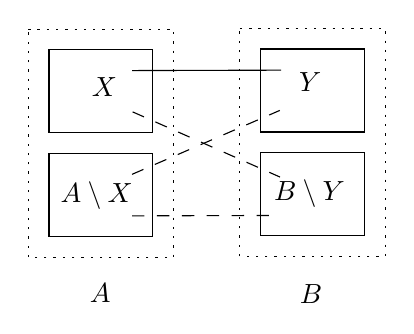
\begin{tikzpicture}[x=0.75pt,y=0.75pt,yscale=-1,xscale=1]
	%uncomment if require: \path (0,300); %set diagram left start at 0, and has height of 300

	%Shape: Rectangle [id:dp6627426419684201]
	\draw  [dash pattern={on 0.84pt off 2.51pt}] (50,60) -- (120,60) -- (120,170) -- (50,170) -- cycle ;
	%Shape: Rectangle [id:dp3761312539244661]
	\draw   (60,70) -- (110,70) -- (110,110) -- (60,110) -- cycle ;
	%Shape: Rectangle [id:dp4675212630222737]
	\draw   (60,120) -- (110,120) -- (110,160) -- (60,160) -- cycle ;
	%Shape: Rectangle [id:dp5057622954470224]
	\draw  [dash pattern={on 0.84pt off 2.51pt}] (152,59.6) -- (222,59.6) -- (222,169.6) -- (152,169.6) -- cycle ;
	%Shape: Rectangle [id:dp43815436760732673]
	\draw   (162,69.6) -- (212,69.6) -- (212,109.6) -- (162,109.6) -- cycle ;
	%Shape: Rectangle [id:dp28652760393509646]
	\draw   (162,119.6) -- (212,119.6) -- (212,159.6) -- (162,159.6) -- cycle ;
	%Straight Lines [id:da24802555849916097]
	\draw    (100,80) -- (171.8,79.8) ;
	%Straight Lines [id:da8218556337757607]
	\draw  [dash pattern={on 4.5pt off 4.5pt}]  (100,150) -- (171.8,149.8) ;
	%Straight Lines [id:da37241741334903355]
	\draw  [dash pattern={on 4.5pt off 4.5pt}]  (100.3,99.9) -- (171.3,131.3) ;
	%Straight Lines [id:da19373579144542075]
	\draw  [dash pattern={on 4.5pt off 4.5pt}]  (100,130) -- (171.2,99.2) ;

	% Text Node
	\draw (79.4,82) node [anchor=north west][inner sep=0.75pt]    {$X$};
	% Text Node
	\draw (64.4,132.4) node [anchor=north west][inner sep=0.75pt]    {$A\setminus X$};
	% Text Node
	\draw (179.2,79.6) node [anchor=north west][inner sep=0.75pt]    {$Y$};
	% Text Node
	\draw (167.2,131.2) node [anchor=north west][inner sep=0.75pt]    {$B\setminus Y$};
	% Text Node
	\draw (78.4,181.6) node [anchor=north west][inner sep=0.75pt]    {$A$};
	% Text Node
	\draw (179.6,182) node [anchor=north west][inner sep=0.75pt]    {$B$};


	\end{tikzpicture}
	\caption{Each line represents all edges between the sets it joins. Edges represented by the solid line is given. Maximum is attained when all edges represented by the dotted line is present. Minimum is attained when no edge of represented by dotted lines are given.}
\end{marginfigure}
\begin{align}
	e(X,B\setminus Y)\leq (|X|)(|B|-|Y|)\\
	e(A\setminus X,Y)\leq(|A|-|X|)(|Y|)\\
	e(A\setminus X,B\setminus Y)\leq (|A|-|X|)(|B|-|Y|)
\end{align}
Where maximum is attained when all the respective edges are drawn.
Putting in eqn4 and simplifying we get:
\begin{align}
 d_1|A||B|&=e(X,Y)+|A||B|-|X||Y|\\
 \Rightarrow d_1|A||B|&=d'|X||Y|+|A||B|-|X||Y|=|A||B|-(1-d')|X||Y|\\
 d_1&=1-(1-d')\left(\frac{|X|}{|A|}\right)\left(\frac{|Y|}{|B|}\right)
\end{align}
We know $1\geq\left(\frac{|X|}{|A|}\right),\left(\frac{|Y|}{|B|}\right)\geq 1-\delta$. From this we get $d_1\geq d'$. Therefore,
\begin{align}
	\begin{split}
	|d_1-d'|&=d_1-d'\\
	&\leq 1-(1-d')\left(\frac{|X|}{|A|}\right)\left(\frac{|Y|}{|B|}\right)-d'\\
	&\leq 1-(1-d')(1-\delta)^2-d'\\
	&\leq (1-d')\left(1-(1-\delta)^2\right)\\
	&\leq \left(1-(1-\delta)^2\right)\\
	&\leq 2\delta-\delta^2\leq 2\delta
	\end{split}
\end{align}
Now we prove it when $d(A,B)=d_2$ is minimum. This occurs when each term of eqn4 attains minimum value. $e(X,Y)$ is fixed. For the other terms the mnimum value attained is 0. Therefore,
\begin{align}
	d_2|A||B|&=e(X,Y)=d'|X||Y|\\
\Rightarrow d_2&=d'\left(\frac{|X|}{|A|}\right)\left(\frac{|Y|}{|B|}\right)
\end{align}
From the bounds of $\left(\frac{|X|}{|A|}\right),\left(\frac{|Y|}{|B|}\right)$ we get $d_2\leq d'$. Therefore, 
\begin{align}
	\begin{split}
		|d_2-d'|&=d'-d_2\\
		&=d'-d'\left(\frac{|X|}{|A|}\right)\left(\frac{|Y|}{|B|}\right)\\
		&=d'\left(1-\left(\frac{|X|}{|A|}\right)\left(\frac{|Y|}{|B|}\right)\right)\\
		&\leq d'\left(1-(1-\delta)^2\right)\\
		&\leq 2\delta-\delta^2\leq 2\delta
	\end{split}
\end{align}
\marginnote{Theorem 2 essentially tells that large subsets of two graph mimics the connectivity of the parent graph}
Since the inequality is proved for maximum and minimum values of $d(A,B)$, we can use lemma 1 to conclude 
\begin{align*}
	|d(A,B)-d(X,Y)|\leq 2\delta
\end{align*}
And from thsi it follows that:
\begin{align*}
	|d(A,B)^2-d(X,Y)^2|\leq |d(A,B)-d(X,Y)||d(A,B)+d(X,Y)|\leq 2\delta(1+1)=4\delta
\end{align*}
\end{proof}

\begin{definition}[$\epsilon$-Regularity]
	We say $A,B$ are epsilon regular if for $X\subseteq A$ and $Y\subseteq B$ with $|X|\geq\epsilon|A|$ and $|Y|\geq\epsilon|B|$ we have $|d(A,B)-d(X,Y)|\leq \epsilon$
\end{definition}











\bibliography{sample-handout}
\bibliographystyle{plainnat}



\end{document}